\chapter{Results}

In this chapter the accuracy of the RCM point when performing injections at different sites on the inner surface of the eye will be evaluated using the method described in \ref{Setup}. Additionally, the choice of control parameters for the augmented Jacobian method will be discussed.

\section{Accuracy of the Jacobian Pseudoinverse Method} \label{Acc_PI}

\subsection{Choosing the Matrix K} \label{K}
When controlling the motion of the tool with the augmented Jacobian matrix, two parameters should be optimized: the control matrix \textbf{K} and the step size of the robot s which determines the magnitude of the change in joint positions for each iteration. Recalling Eqn. \ref{K_J}, we can see that each entry in \textbf{K} gives a weight to the error of one component in the pose, i.e. if one entry in \textbf{K} is large, the error in that component will converge to zero faster. On the other hand, two of the components in the pose vector are angles in radians, while the others are cartesian positions given in meters. The Jacobian matrix does not 'know' about these different length scales, thus the matrix \textbf{K} needs to correct for it. Additionally, the two angles have different levers with respect to the needle tip position, i.e. a change of 0.1 radians for both angles will result in a different displacement of the needle tip in y and z direction.  As a rough correction for this, we can calculate the approximate change in the position of the tip per angle of the robot is in its initial configuration ($q_i = 0$). 
For a small change of angle in $q_1$ and $q_3$, the change of the z- and y-position of the needle tip is given by 
\begin{align*}
\Delta z&=\sin\Delta q_1 \sqrt{l_2^2+l_6^2}\\
\Delta y&=\sin\Delta q_1 \sqrt{l_5^2+l_6^2}
\end{align*}
This gives us an approximate correction factor of 10 for the entries of \textbf{K} corresponding to the angular errors. Thus, we start optimization with \textbf{K}=diag([1, 10, 10, 1, 1, 1]). 

\subsection{Error in the RCM Position}

In Section \ref{control} a control loop was introduced which iterates until the robot's current pose matches a given target pose within a predefined magnitude. Large distances between start and target pose require a high number of iterations to converge because the Jacobian matrix attempts to correct the parameter with the largest error in one iteration, thereby displacing the other parameters heavily. These then return to their desired values in subsequent iterations as illustrated in Figure \ref{large_step}. This behaviour can be efficiently suppressed by splitting the full trajectory into several smaller parts. If the distance between these intermediate target positions is sufficiently small the control loop will converge from one position to the next within a small number of iterations without excessive overshooting.

\begin{algorithm}[t!]
 \begin{algorithmic}[1]
  \STATE $\textbf{start\_pose} \leftarrow \textit{get\_task\_pose}()$
  \STATE $\textbf{total\_distance} \leftarrow \textbf{target\_pose} - \textbf{start\_pose}$
  \STATE $\textbf{step} \leftarrow \textbf{total\_distance} / abs(\textbf{total\_distance}) \cdot \text{step\_size}$
  \WHILE {$max(abs(\textbf{target\_pose}-\textbf{current\_pose})) > 0.0003$}
   \STATE $\textbf{intermediate\_target\_position} \leftarrow \textbf{current\_pose} + \textbf{step}$
   \STATE $\text{Control\_Loop}(\bm{K}, \textbf{intermediate\_target\_position}, J_a, \lambda)$
   \STATE $\textbf{current\_pose} \leftarrow \textit{get\_task\_pose}()$
   \ENDWHILE 
 \end{algorithmic}
 \caption{$\text{Extended\_Control\_Loop}(\textbf{target\_pose}, \text{step\_size})$}
 \label{alg:ext_control_loop}
\end{algorithm}

\begin{figure}[b!]
	\begin{center}
		%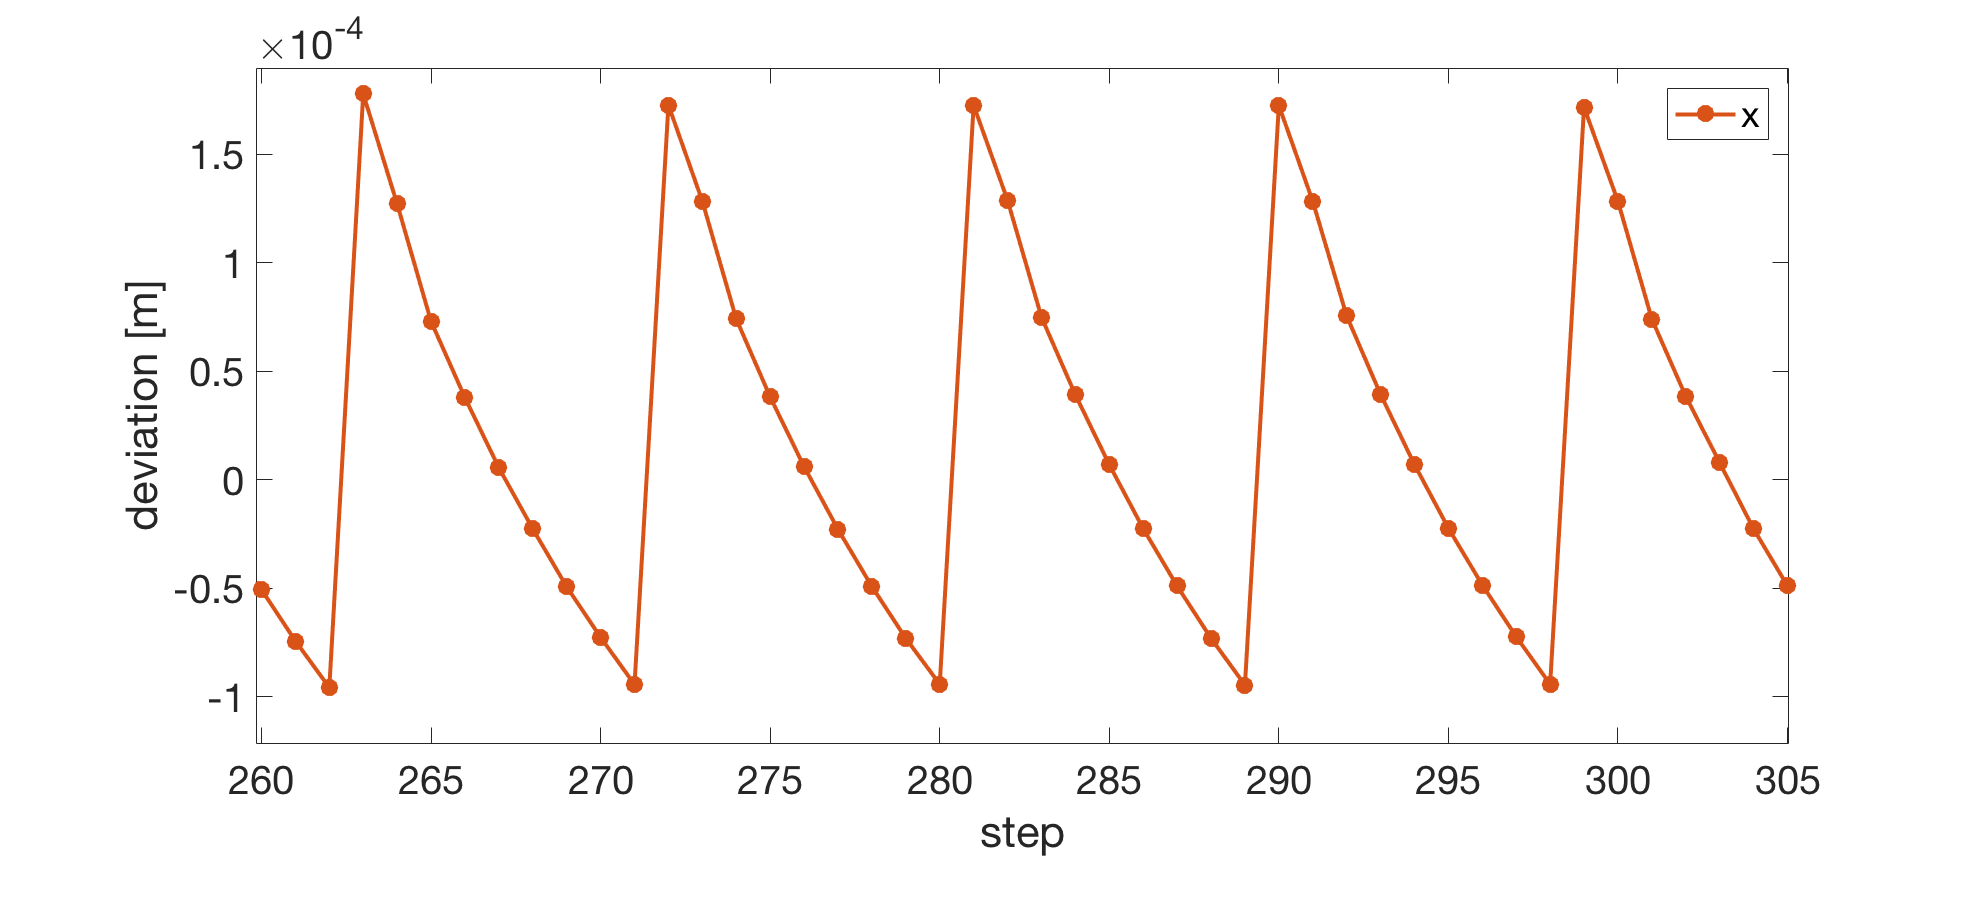
\includegraphics[width=15cm]{large_step}
		\import{images/}{large_step_tex.pdf_tex}
		\caption{Error in the RCM position when performing a step that is too large. The step starts with a large displacement in one direction and requires many iterations of the control loop to return to the desired RCM position.}
		\label{large_step}
	\end{center}
\end{figure}

The process of splitting the trajectory is illustrated in Algorithm \ref{alg:ext_control_loop}. given a target pose that is far away from the current pose, the extended control loop splits the trajectory in many small steps of equal length, determined by the step size. For each small step, the control loop presented in Section \ref{control} is executed, which brings the needle from the current position sufficiently close to the intermediate target. After the intermediate target is reached, a new small step in the direction of the target pose is calculated and again executed by the first control loop presented in Section \ref{control}.

\begin{figure}[b!]
	\begin{center}
		%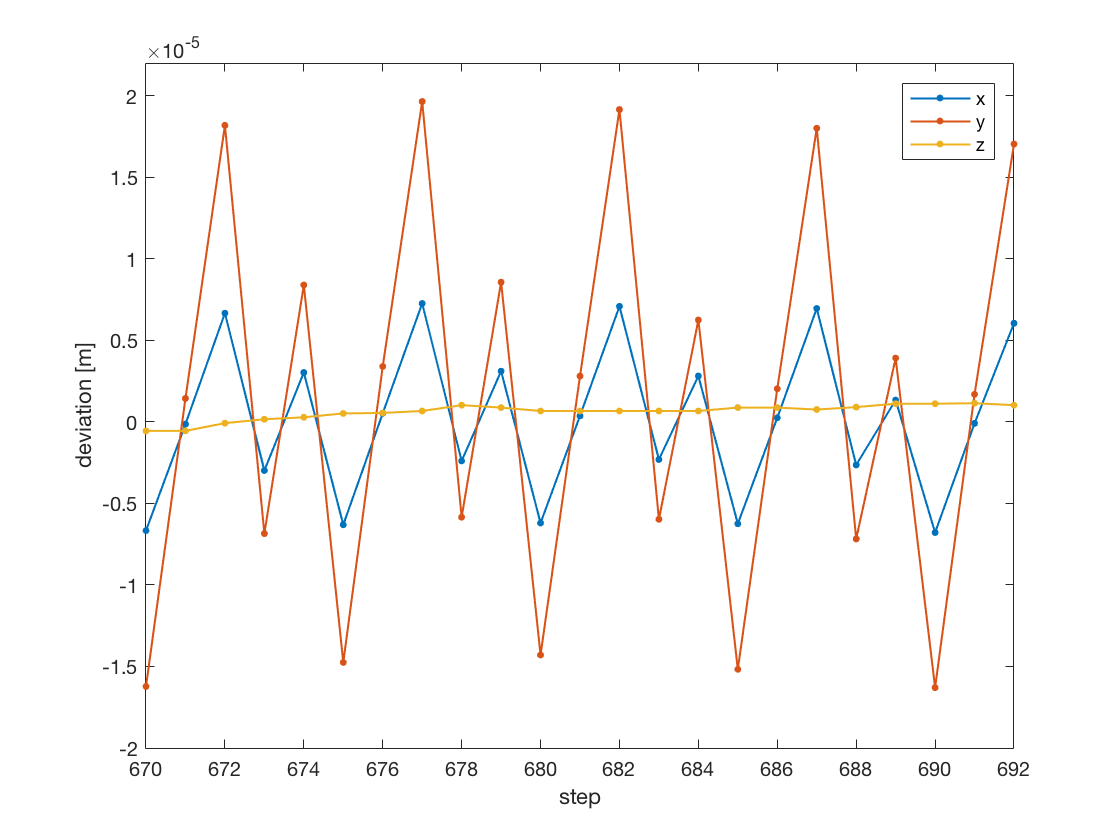
\includegraphics[width=15cm]{alignment_error_section_png}
		\import{images/}{alignment_error_section_refactored.pdf_tex}
		\caption{Error in the RCM position during 22 iterations of pivoting the needle around its tip during the alignment process described in Section \ref{Setup}.}
		\label{error_align_overall}
	\end{center}
\end{figure}

As an example for a proper choice in step size, two parts of the injection process are shown: The alignment of the needle with the trocar (at point 2 in Section \ref{Setup}), in which the RCM point is positioned at the needle tip ($\lambda=1$) and the entire robot pivots around its tip, as well as the movement from point 3 to point 7. These two were chosen because one illustrates the 'worst case' in terms of keeping the RCM point steady (as a small angle change leads to a large displacement of the RCM due to the long lever) and the other requires simultaneous adjustment of both angles of the needle while maintaining the RCM point.

Figure \ref{error_align_overall} shows the overall position of the RCM point during the alignment process. 500 steps according to the control loop in Section \ref{control} were performed to correct the angles $\Phi$ and $\Psi$ by $0.0048$ rad ($\approx 0.28$ deg) and $0.212$ rad ($\approx 12.12$ deg), respectively. In each of these steps, roughly 3 iterations were needed to ensure the accuracy of the RCM, resulting in a total of 1350 data points. The total computation time for this section of the injection process was about 3 minutes, which is quite a lot but was required to reach a high precision for the RCM point. During many iterations of this injection step, $K=diag([1 10 12 1 2 2])$ proved to be a good choice for the control matrix as a compromise between speed and accuracy.

\begin{figure}[b!]
	\begin{center}
		%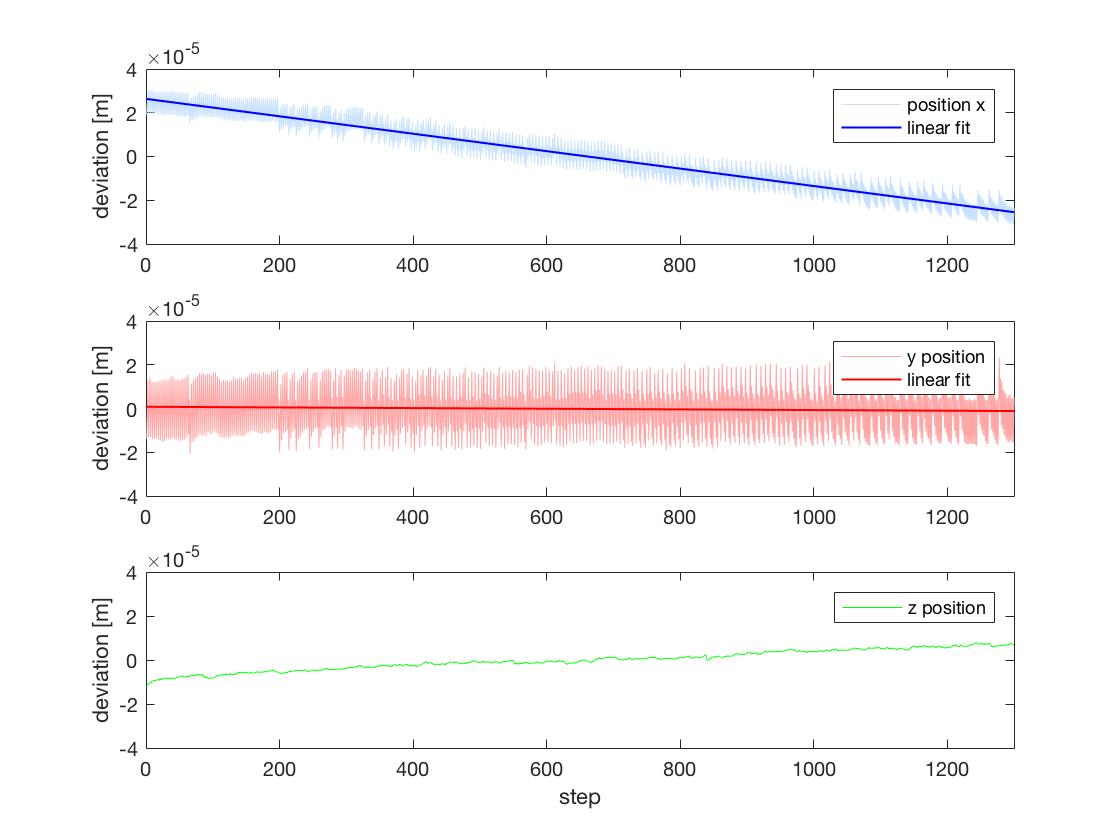
\includegraphics[width=15cm]{drift}
		\import{images/}{drift_tex.pdf_tex}
		\caption{ Overall error in the RCM position for the alignment of the needle with the trocar as proposed in Section \ref{Setup}. }
		\label{error_align}
	\end{center}
\end{figure}

The first thing to note about Figure \ref{error_align_overall} is that both $y_{rcm}$ and $z_{rcm}$ remain roughly constant during the entire procedure while $x_{rcm}$ experiences some drift. This drift occurs only in x-direction because the weight in $\bm{K}$ associated with $x_{rcm}$ is only half as large as the weights associated with $y_{rcm}$ and $z_{rcm}$.  When adjusting the values in $\bm{K}$, it is always necessary to find a good trade-off between accuracy of the RCM position and computation speed. By setting the weight related to $x_{rcm}$ to 2 instead of 1 the drift is reduced but the needle pose converges to the target pose much slower because the change in x-position competes with the change in both $\Psi$ and $\Phi$. In this example, the drift of $x_{rcm}$ during the alignment process is only $\pm3\cdot10^{-5}m$ which is negligible compared to the radius of the trocar which is about $45\cdot10^{-5}m$.

Both Figure \ref{error_align_overall} and \ref{error_align} illustrate the influence of the step size on the accuracy of the RCM point. A total of 500 steps are performed to align the needle with the trocar, but one of the initial angles is much closer to the target angle than the other. As a  result one angle will have a larger error each step and the Jacobian will calculate a larger $\Delta L$ to correct the angle, thus displacing the RCM more in one direction than the other. In this example the error in angle $\Psi$ is large, thus each step the needle will rotate about the z-axis by a large amount and as a result displace the RCM point in y direction. the error in angle $\Phi$ is very small and thus the RCM is hardly displaced in z-position. The x-position, which roughly corresponds to the depth the needle is injected into the eye, is affected by both angle changes, therefore its error is somewhere in between.

Figures \ref{3_7} and \ref{3_7_drift} show the error per step and the overall drift and  for the RCM point during the movement from point $3$ to point $7$ proposed in Section \ref{Setup}. Both are very similar in precision to the ones for the alignment with the trocar which shows that simultaneous adjustment of two angles does not significantly decrease performance. The total computation time for this section of the injection was roughly 2 minutes. 

 \begin{figure}[t!]
	\begin{center}
		%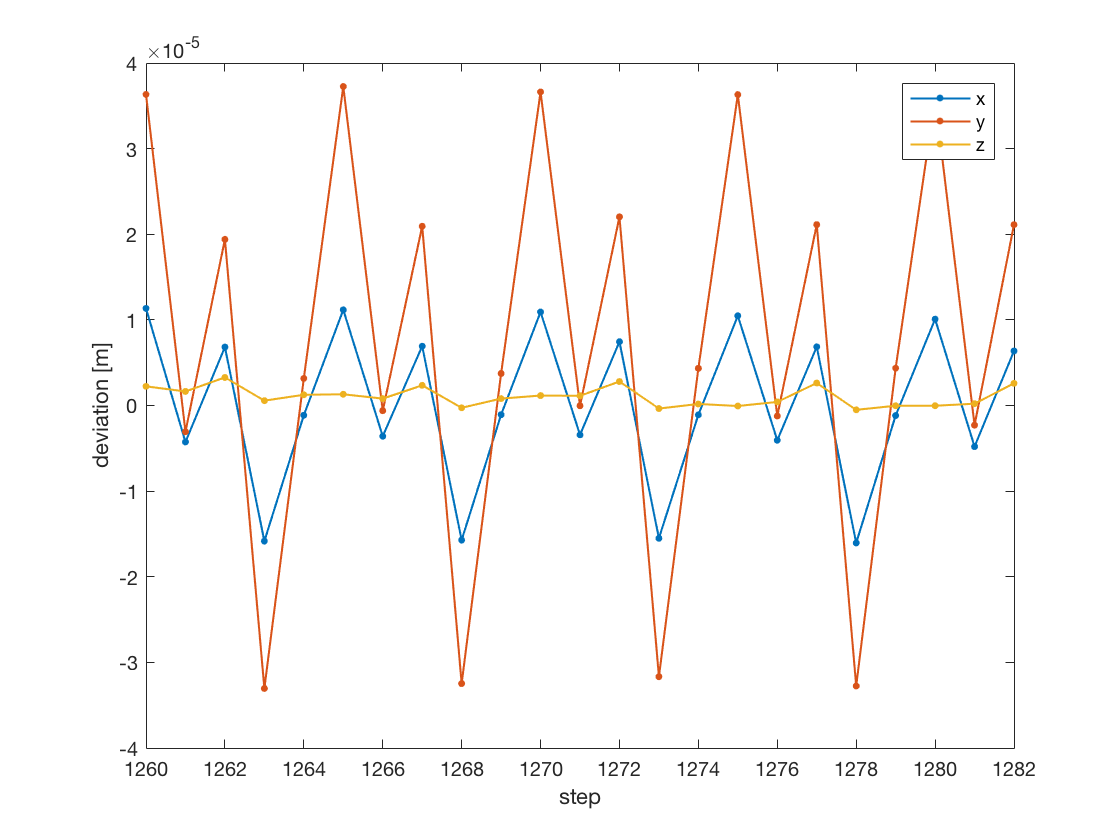
\includegraphics[width=15cm]{3_7}
		\import{images/}{3_7_tex.pdf_tex}
		\caption{ Error in the RCM position during 22 iterations of the movement  from point $3$ to point $7$ as proposed in Section \ref{Setup}.}
		\label{3_7}
	\end{center}
\end{figure}

\begin{figure}[t!]
	\begin{center}
		%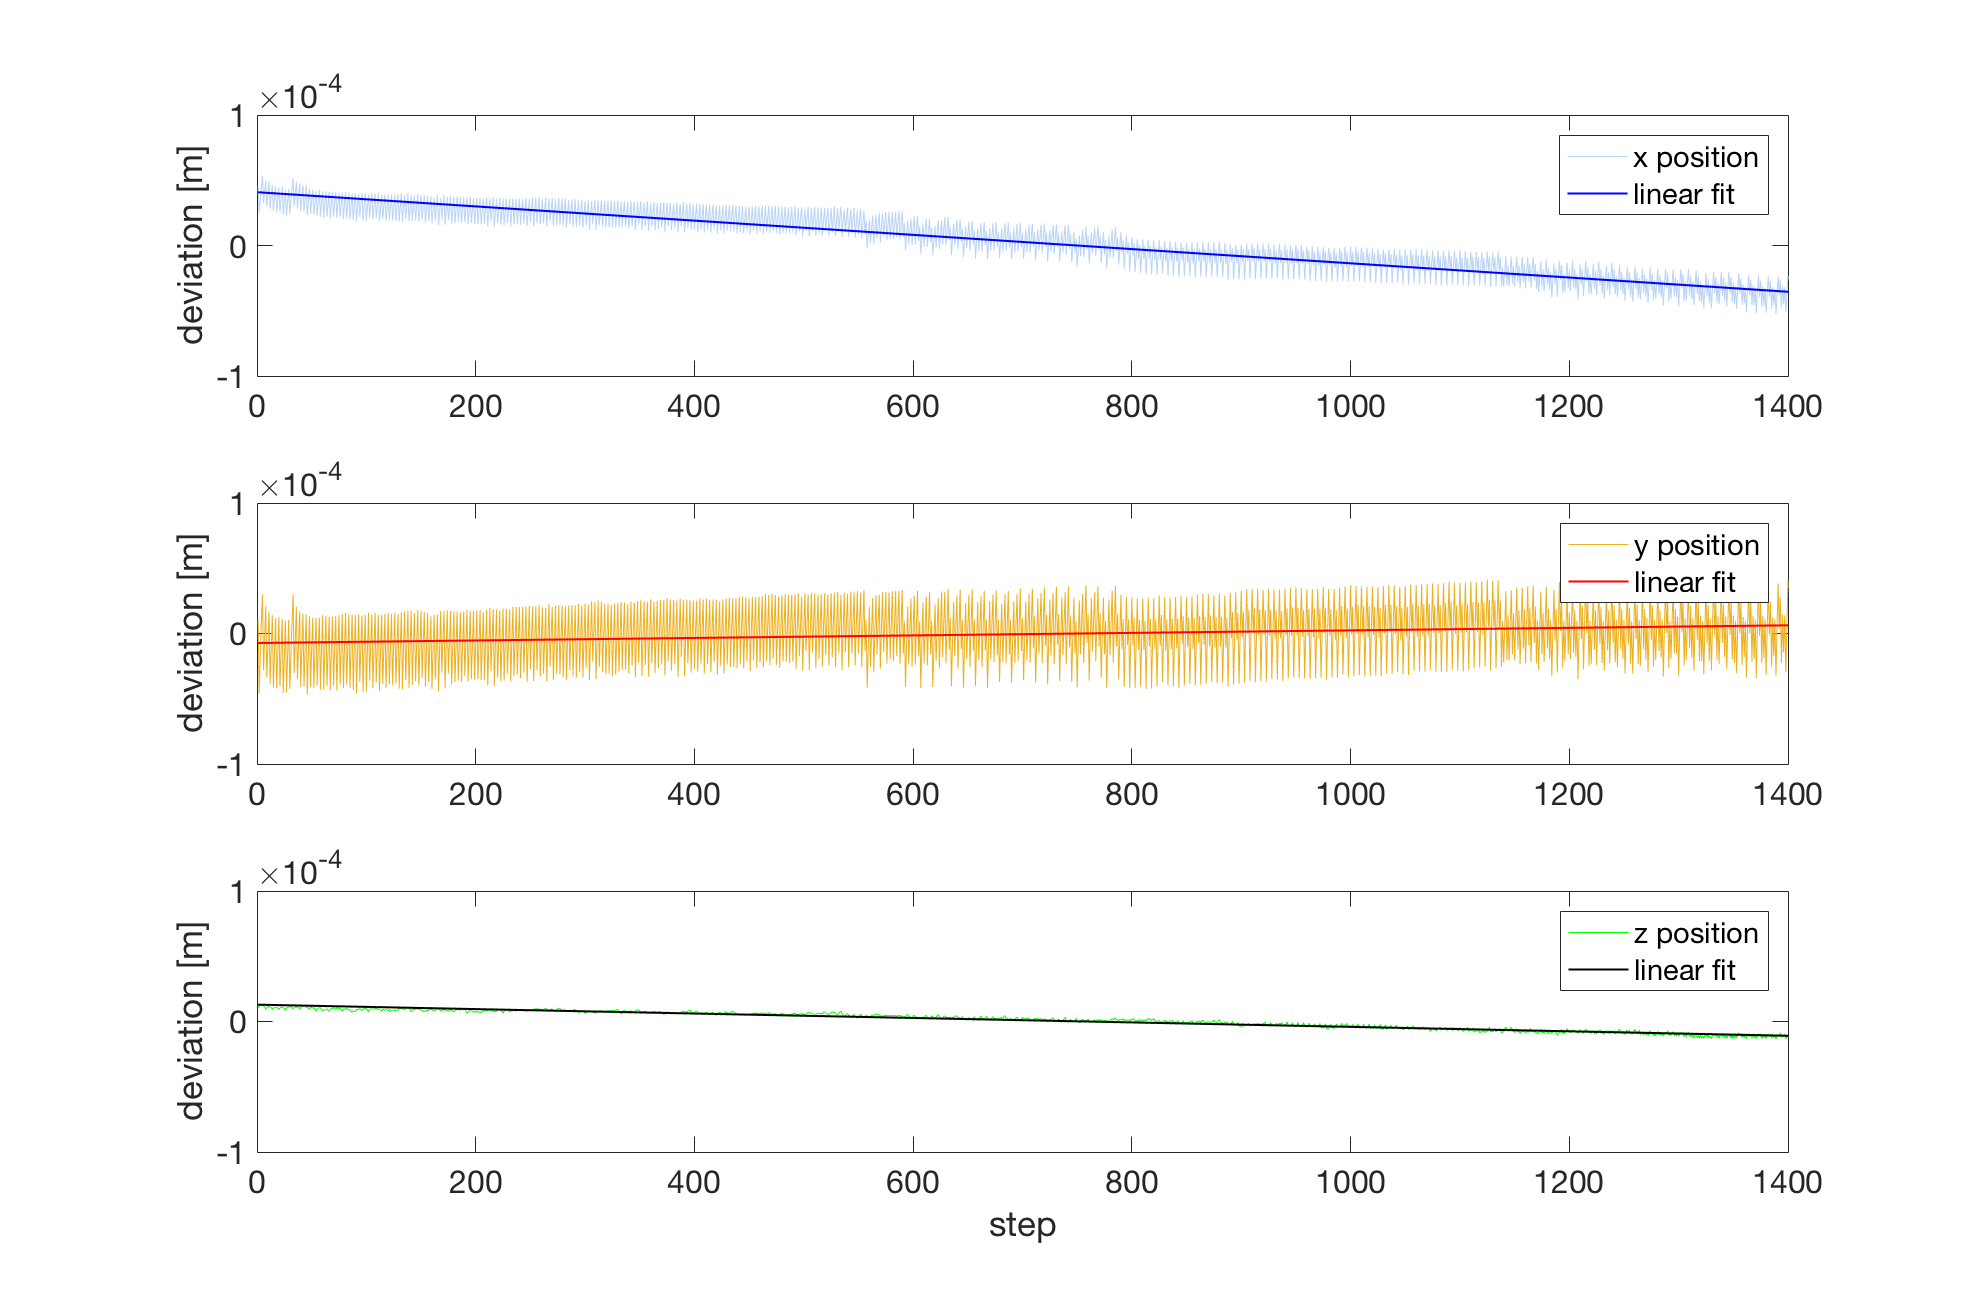
\includegraphics[width=15cm]{3_7_drift}
		\import{images/}{3_7_drift_tex.pdf_tex}
		\caption{ Overall error in the RCM position for the movement from point $3$ to point $7$ as proposed in Section \ref{Setup}. }
		\label{3_7_drift}
	\end{center}
\end{figure}

\section{Accuracy of the Dampened Least Squares Method} \label{Acc_DLS}

This section discusses the accuracy of V-REPs inverse kinematic solver which utilizes the Levenberg-Marquardt algorithm discussed in Section \ref{DLS}. The DLS algorithm functions very similarly to the Jacobian pseudoinverse method in that it linearises the IK problem near the current pose via the Jacobian matrix. There are two key points in which the DLS algorithm improves upon the Jacobian pseudoinverse approach: Firstly, the DLS algorithm introduces the damping parameter $D$ which prevents the algorithm from running into numeric instability close to a singularity. Secondly, the DLS algorithm never performs a matrix inversion, improving its computation time especially for Manipulators with a large number of links.
For the robot considered in this thesis, the DLS algorithm should not have a significantly higher performance than the pseudoinverse method, given an optimal choice for the matrix $\bm{K}$ and a sufficiently small step size, because there are no singularities in the workspace of the robot. Thus, to give an idea about the precision that is possible to achieve with the augmented Jacobian method the precision of the built-in IK solver is evaluated. Figure \ref{DLS_method} shows the setup used for showcasing the precision of the Dampened Least Squares Method. An off-axis spiral is drawn with the needle tip, keeping the RCM point steady at all times. Figure \ref{DLS_result} shows the deviation of the RCM point. The damping factor $D$ is set to 0.1.  

\begin{figure}[h!]
	\begin{center}
		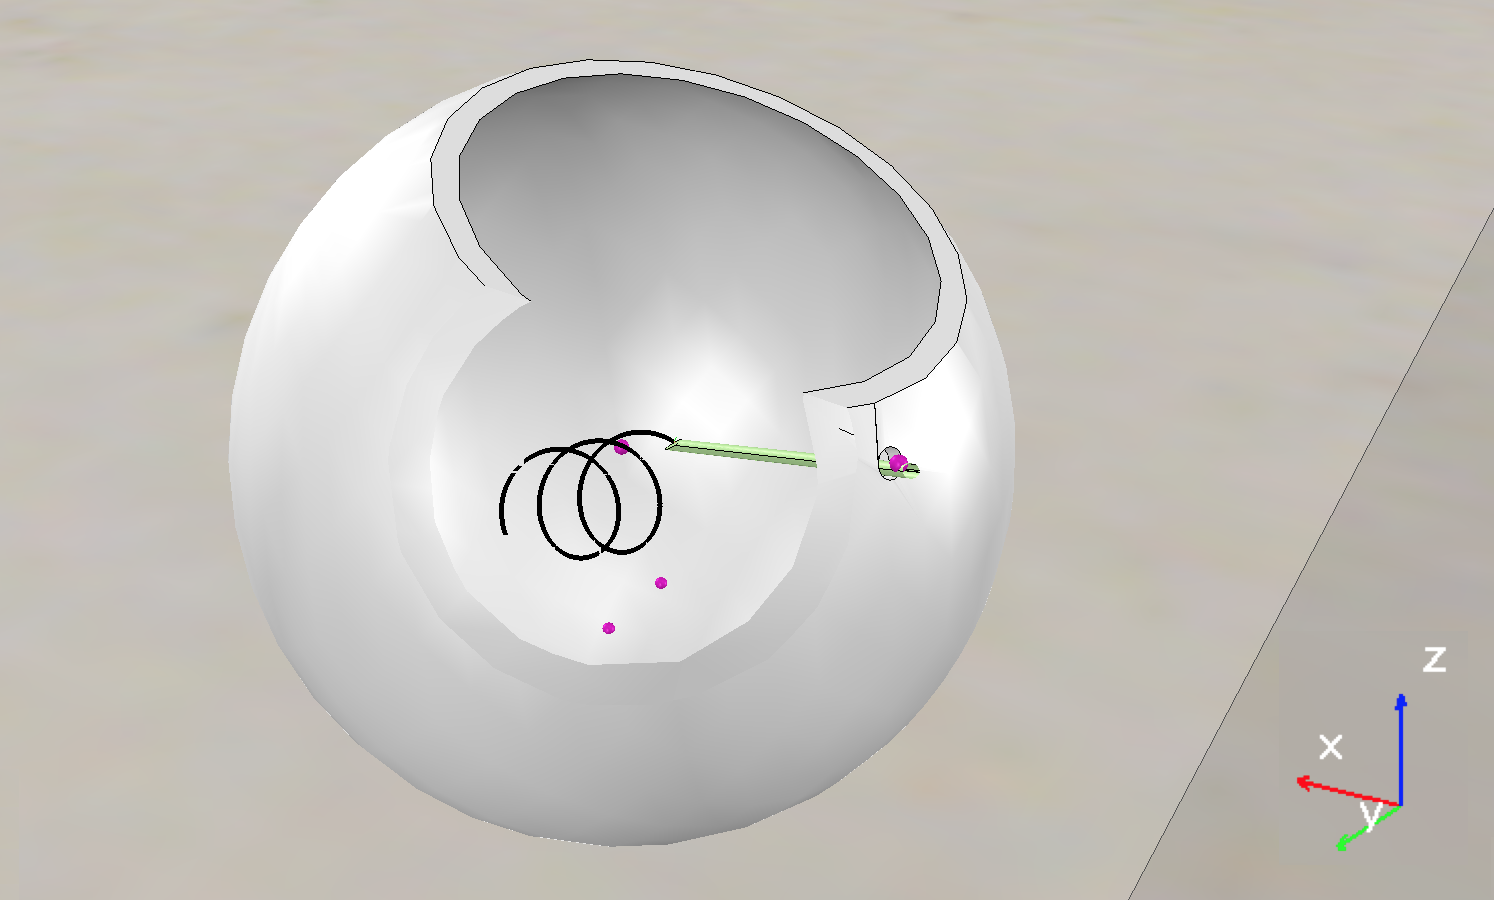
\includegraphics[width=15cm]{vrep-benchmark}
		\caption{Needle tip of the Robot tracing the shape of a spiral within the eye while keeping the RCM point steady, using V-REPs inverse kinematics module. The trajectory was recorded by V-REP using a graph object positioned at the needle tip. }
		\label{DLS_method}
	\end{center}
\end{figure}

\begin{figure}[h!]
	\begin{center}
		%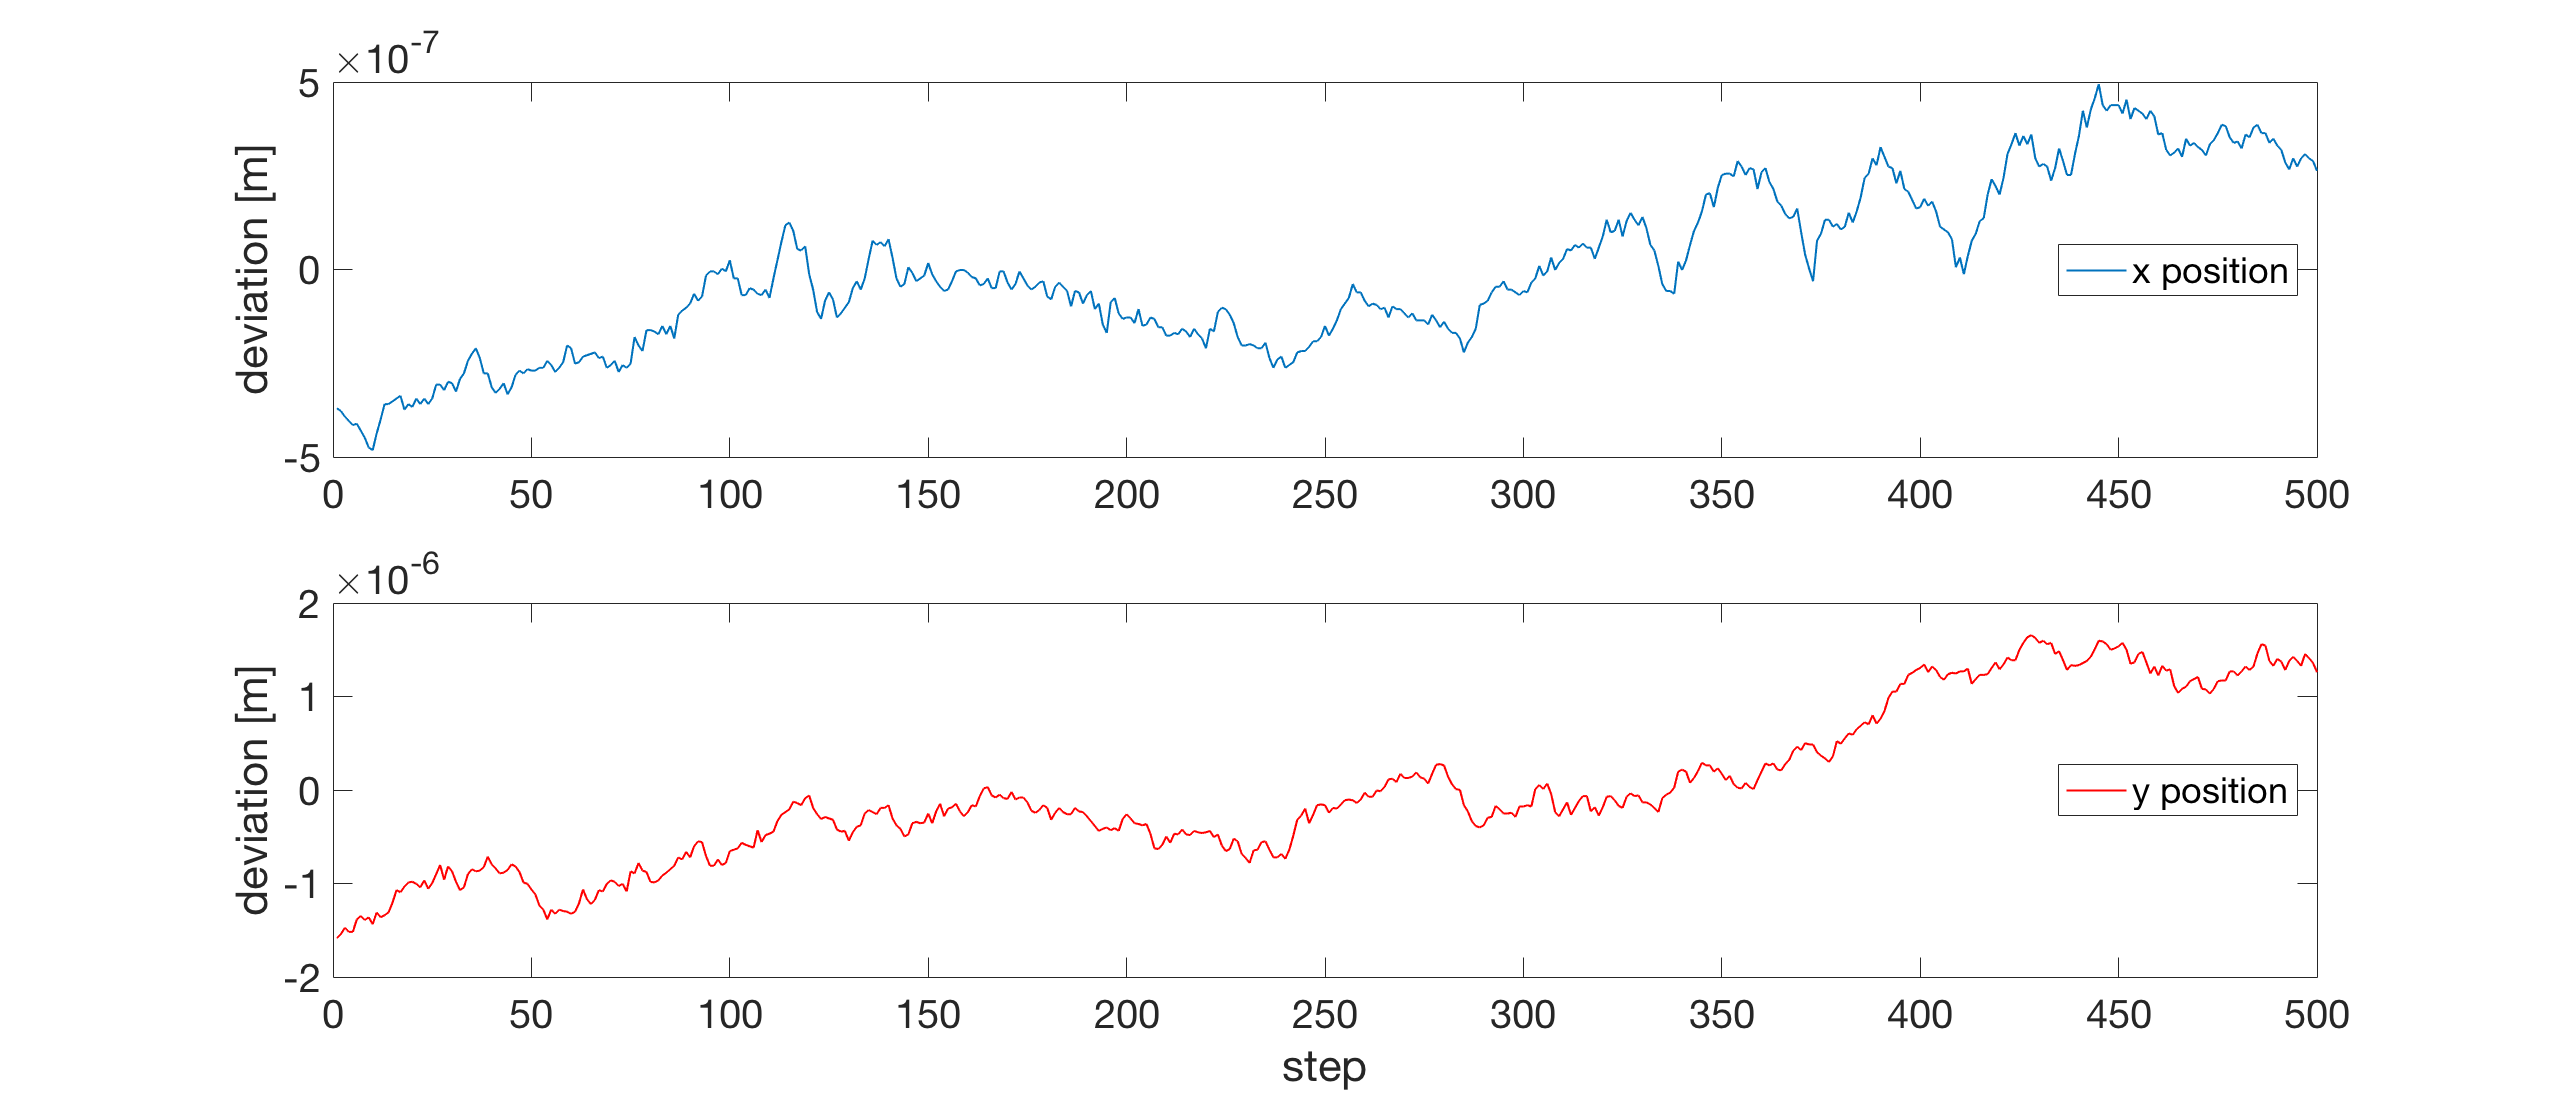
\includegraphics[width=16cm]{IK_solution}
		\import{images/}{IK_solution_tex.pdf_tex}
		\caption{Error in the RCM position during the first 500 calculation steps of the V-REP IK solver, producing the trajectory seen in Figure \ref{DLS_method}.}
		\label{DLS_result}
	\end{center}
\end{figure}

The accuracy of the DLS method proved to be extremely high compared to the Jacobian pseudoinverse method. Furthermore, the computation time to draw the shape in Figure \ref{DLS_method} was only 28 seconds. although the minimum precision was set to 0.1mm, the method seemed to be much more precise, implying that a smaller damping factor could have been chosen to speed up computation even more. 